\verb|RobustNeuralNetwork.jl| contains two classes of neural network models: RENs and LBDNs. This section gives a brief overview of the two model architectures and how they are parameterized to automatically satisfy robustness certificates. We also provide some background on the different types of robustness metrics used to construct the models.

% Model types
\subsection{What are RENs and LBDNs?} \label{sec:model-structures}

A \textit{Lipschitz-Bounded Deep Network} (LBDN) is a (memoryless) deep neural network with a built-in upper-bound on its Lipschitz constant (Sec. \ref{sec:robustness-lipschitz}). Suppose the network has inputs $u \in\mathbb{R}^{n_u}$, outputs $y \in \mathbb{R}^{n_y}$, and hidden units $z_k \in \mathbb{R}^{n_k}$. The structure of an LBDNs is a $L$-layer feed-forward network (like an MLP or CNN)
\begin{align} 
z_0 &= x \label{eqn:lbdn-z0}\\
z_{k+1} &= \sigma(W_k z_k + b_k), \quad k = 0, \ldots, L-1 \label{eqn:lbdn-sandwich}\\
y &= W_L z_L + b_L, \label{eqn:lbdn-output}
\end{align}
where the $W_k, b_k$ are the layer weights and biases (respectively), and $\sigma$ is a nonlinear activation function (e.g. $\tanh$, ReLU).

A \textit{Recurrent Equilibrium Network} (REN) is a recurrent model (with memory) described by a linear dynamical system in feedback with a nonlinear activation function. Writing $x_t \in \mathbb{R}^{n_x}$ for the internal states of the system, a REN can be expressed mathematically as
\begin{align}
    \begin{bmatrix}
        x_{t+1} \\ v_t \\ y_t
    \end{bmatrix}&=
    \overset{W}{\overbrace{
    		\left[
    		\begin{array}{c|cc}
    		A & B_1 & B_2 \\ \hline 
    		C_{1} & D_{11} & D_{12} \\
    		C_{2} & D_{21} & D_{22}
    		\end{array} 
    		\right]
    }}
    \begin{bmatrix}
        x_t \\ w_t \\ u_t
    \end{bmatrix}+
    \overset{b}{\overbrace{
    		\begin{bmatrix}
    		b_x \\ b_v \\ b_y
    		\end{bmatrix}
    }}, \label{eqn:ren-G}\\
    w_t=\sigma(&v_t):=\begin{bmatrix}
    \sigma(v_{t}^1) & \sigma(v_{t}^2) & \cdots & \sigma(v_{t}^q)
    \end{bmatrix}^\top, \label{eqn:ren-sigma}
\end{align}
where $v_t, w_t \in \mathbb{R}^{n_v}$ are the inputs and outputs of the activation function $\sigma$. Graphically, this is equivalent to Figure \ref{fig:ren}, where the linear system $G$ is given by Equation \ref{eqn:ren-G}.

\begin{figure}[h]
    \centering
    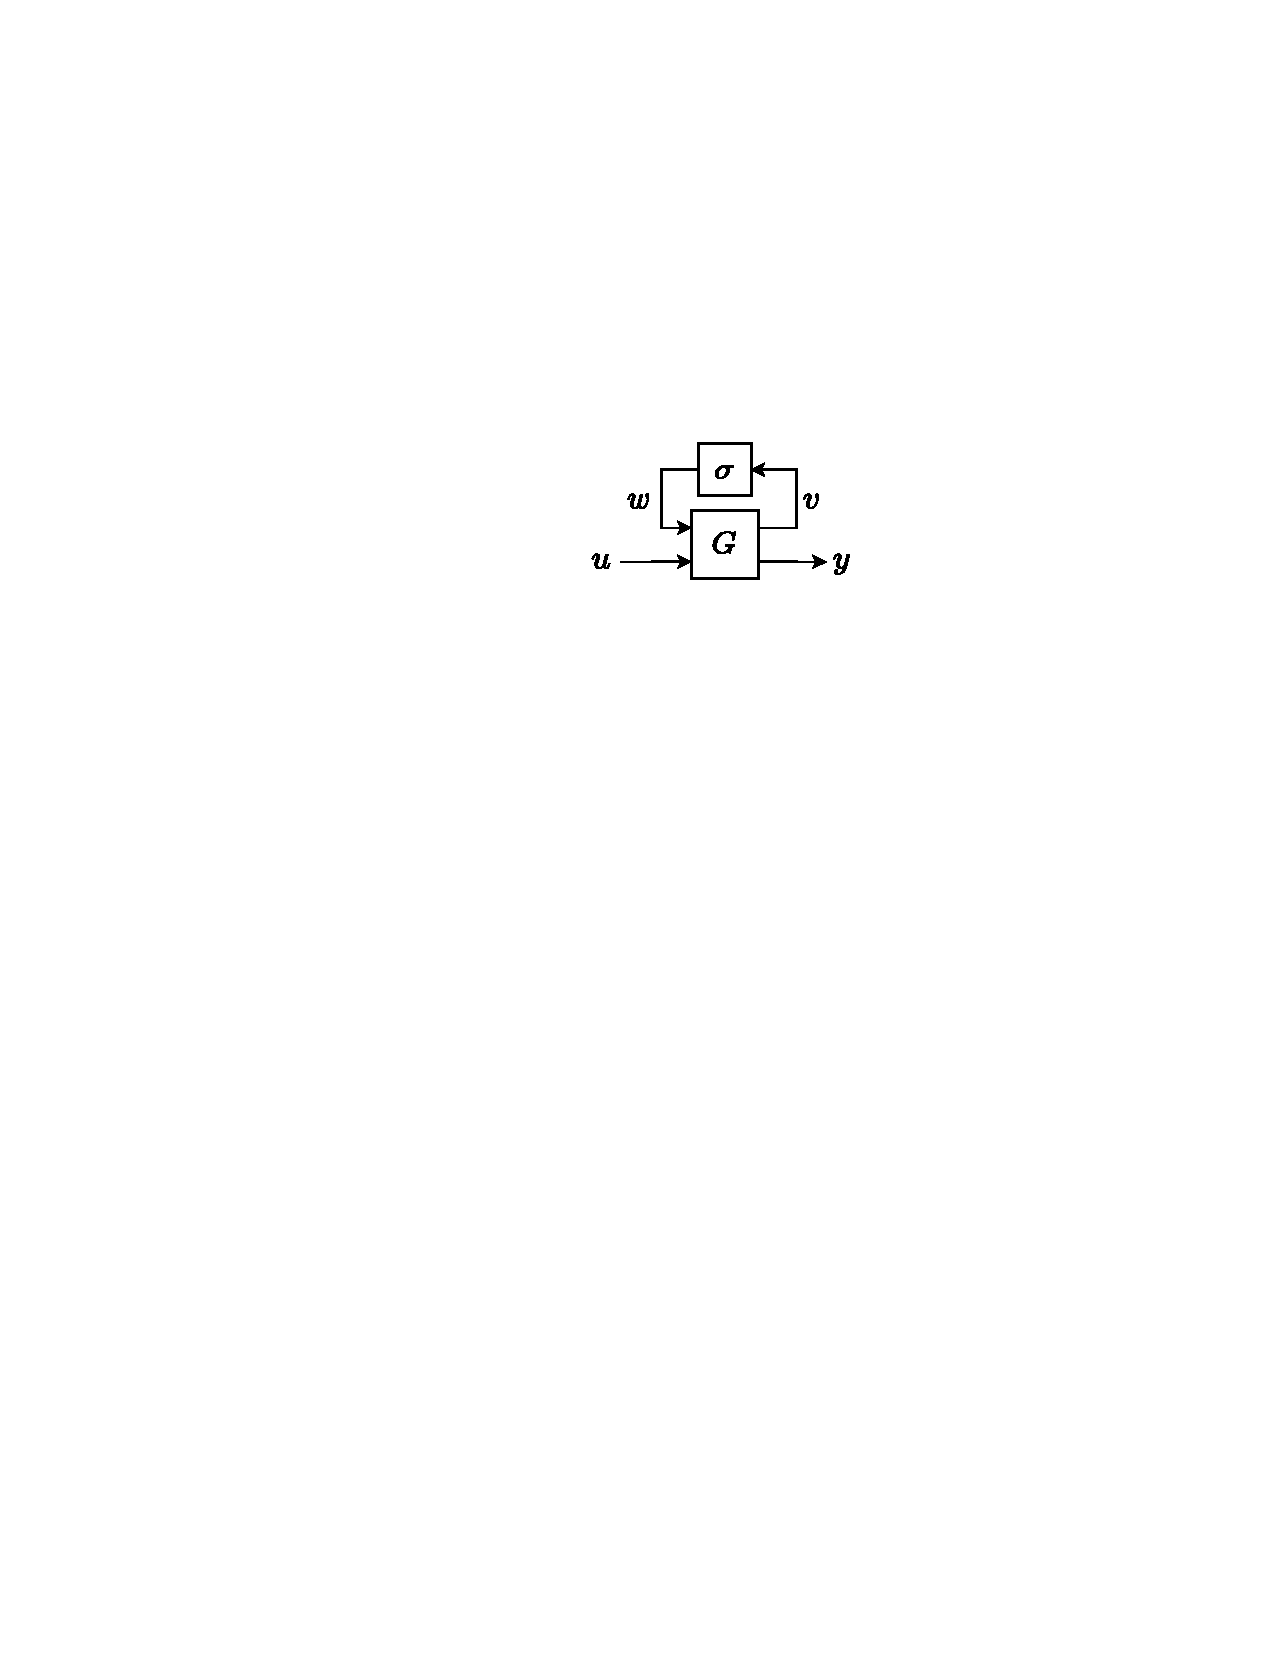
\includegraphics[width=0.19\textwidth]{Images/ren.pdf}
    \vspace{-2mm}
    \caption{Feedback structure of a recurrent equilibrium network.}
    \label{fig:ren}
\end{figure}

See \cite{Revay++2023} and \cite{Wang+Manchester2023} for more on RENs and LBDNs, respectively.

\begin{remark}
	\cite{Revay++2023} makes special mention of ``acyclic'' RENs, which have a lower-triangular $D_{11}$ matrix. Acyclic RENs are significantly more efficient to evaluate than RENs with a dense $D_{11}$ matrix, and performance is typically similar across a range of problems. All RENs in \verb|RobustNeuralNetworks.jl| are therefore acyclic RENs.
\end{remark}

% Robustness
\subsection{Robustness metrics and IQCs} \label{sec:robustness}

All neural network models in \verb|RobustNeuralNetworks.jl| are designed to satisfy a set of user-defined robustness constraints. The RENs can satisfy a range of robustness criteria, some relating to the internal dynamics of a model and others relating to its input-output map. LBDNs are more specialized and are specifically constructed to have a finite, user-tunable Lipschitz bound (Sec. \ref{sec:robustness-lipschitz}).

\subsubsection{Contracting systems} \label{sec:robustness-contraction}

Firstly, all of our RENs are contracting systems. This means that they exponentially ``forget'' their initial conditions. If the system starts at two different initial conditions but is given the same input sequence, the internal states will exponentially converge over time. Figure \ref{fig:contracting-ren} shows an example of a contracting REN with one input and a single internal state, where two simulations of the system start with different initial conditions but are provided the same sinusoidal input. See \cite{Bullo2022} for a detailed introduction to contraction theory for dynamical systems.

\begin{figure}[ht]
    \centering
    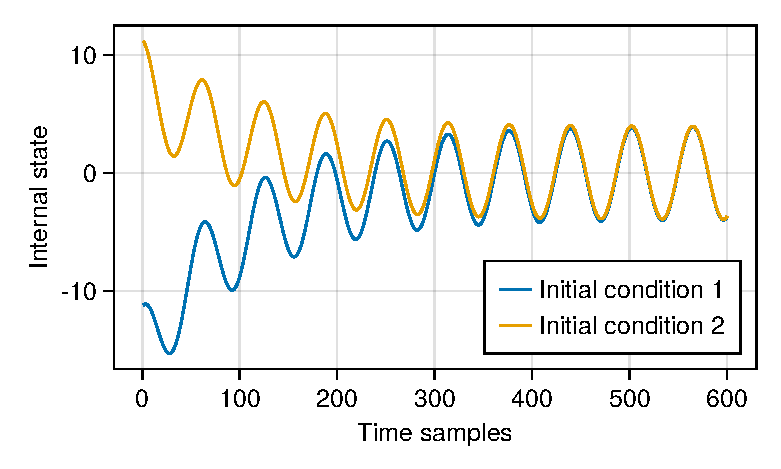
\includegraphics[width=0.47\textwidth]{Images/contracting_ren.pdf}
    \caption{Simulation of a contracting REN with a single internal state. The system is simulated from two different initial states with the same sinusoidal input. The contracting system exponentially forgets its initial condition.}
    \label{fig:contracting-ren}
\end{figure}

\subsubsection{Incremental IQCs}

We define additional robustness criteria on the input-output map of RENs with incremental \textit{integral quadratic constraints} (IQCs). Suppose we have a model $\mathcal{M}$ starting at two different initial conditions $a,b$ with two different input signals $u, v$, and consider their corresponding output trajectories $y^a = \mathcal{M}_a(u)$ and $y^b = \mathcal{M}_b(v).$ The model $\mathcal{M}$ satisfies the IQC defined by matrices $(Q, S, R)$ if
\begin{equation}
    \sum_{t=0}^T
    \begin{bmatrix}
        y^a_t - y^b_t \\ u_t - v_t
    \end{bmatrix}^\top
    \begin{bmatrix}
        Q & S^\top \\ S & R
    \end{bmatrix}
    \begin{bmatrix}
        y^a_t - y^b_t \\ u_t - v_t
    \end{bmatrix} 
    \ge -d(a,b)
    \quad \forall \, T
\end{equation}
for some function $d(a,b) \ge 0$ with $d(a,a) = 0$, where $0 \preceq Q \in \mathbb{R}^{n_y\times n_y}$, $S\in\mathbb{R}^{n_u\times n_y},$ $R=R^\top \in \mathbb{R}^{n_u\times n_u}.$ 

In general, the IQC matrices $(Q,S,R)$ can be chosen (or optimized) to meet a range of performance criteria. The following special cases are worth noting.

\subsubsection{Lipschitz bounds (smoothness)} \label{sec:robustness-lipschitz}
If $Q = -\frac{1}{\gamma}I$, $R = \gamma I$, $S = 0$ for some $\gamma \in \mathbb{R}$ with $\gamma > 0$, the model $\mathcal{M}$ satisfies a Lipschitz bound (incremental $\ell_2$-gain bound) of $\gamma$ defined by
\begin{equation}
\|\mathcal{M}_a(u) - \mathcal{M}_b(v)\|^2 \le \gamma^2 \|u - v\|^2
\end{equation}
where $\|\cdot\|$ denotes the $\ell_2$ norm. Qualitatively, the Lipschitz bound is a measure of the network's ``smoothness''. If $\gamma$ is small, then small changes to the inputs $u,v$ induce only small changes to the model output. If $\gamma$ is large (or unbounded, as in the case of, e.g., MLPs and CNNs), then the model output can change significantly even with negligible changes to the inputs. This can make the model highly sensitive to noise, adversarial attacks, and other input disturbances.

As the name suggests, all LBDN models are constructed to have a user-tunable (or learnable) Lipschitz bound.

\subsubsection{Incremental passivity} 
We have implemented two versions of incremental passivity. In each case, the network must have the same number of inputs and outputs.

\begin{enumerate}
    \item If $Q = 0, R = -2\nu I, S = I$ where $\nu \ge 0$, the model is incrementally passive (incrementally strictly input passive if $\nu > 0$). Mathematically, the following inequality holds.
    \begin{equation}
    \langle \mathcal{M}_a(u) - \mathcal{M}_b(v), u-v \rangle \ge \nu \| u-v\|^2
    \end{equation}
    \item If $Q = -2\rho I, R = 0, S = I$ where $\rho > 0$, the model is incrementally strictly output passive. Mathematically, the following inequality holds.
    \begin{equation}
    \langle \mathcal{M}_a(u) - \mathcal{M}_b(v), u-v \rangle \ge \rho \| \mathcal{M}_a(u) - \mathcal{M}_b(v)\|^2
    \end{equation}
\end{enumerate}

For more details on IQCs and their use in RENs, please see \cite{Revay++2023}.

% Parameterisations
\subsection{Direct and explicit parameterizations} \label{sec:parameterizations}

The key advantage of the models in \verb|RobustNeuralNetworks.jl| is that they \textit{naturally} satisfy the robustness constraints of Section \ref{sec:robustness} -- i.e., robustness is guaranteed by construction. There is no need to impose additional (possibly computationally-expensive) constraints while training a REN or an LBDN. One can simply use unconstrained optimization methods like gradient descent and be sure that the final model will satisfy the robustness requirements.

We achieve this by constructing the weight matrices and bias vectors in our models to automatically satisfy specific linear matrix inequalities (see \cite{Revay++2023} for details). The learnable parameters of a REN or LBDN are a set of free, unconstrained variables $\theta \in \mathbb{R}^N$. When the set of learnable parameters is exactly $\mathbb{R}^N$ like this, we call the parameterization a \textit{direct parameterization}. Equations \ref{eqn:ren-G} to \ref{eqn:lbdn-output} describe the \textit{explicit parameterizations} of RENs and LBDNs: model structures that can be called and evaluated on data. For a REN, the explicit parameters are $\bar{\theta} := [W, b]$, and for an LBDN they are $\bar{\theta} := [W_0, b_0, \ldots, W_L, b_L]$. The mapping $\theta \mapsto \bar{\theta}$ depends on the specific robustness constraints to be imposed on the explicit model. 
% The direct parameters for RENs and LBDNs are defined in \cite{Revay++2023} and \cite{Wang+Manchester2023}, respectively.

\subsubsection{Implementation} \label{sec:params-implementation}
RENs are defined by two abstract types in \verb|RobustNeuralNetworks.jl|. Subtypes of \verb|AbstractRENParams| hold all the information required to directly parameterize a REN satisfying some robustness properties. For example, to initialize the direct parameters of a \textit{contracting} REN with 1 input, 10 states, 20 neurons, 1 output, and a \texttt{relu} activation function, we use the following. The direct parameters $\theta$ are stored in \verb|model_ps.direct|. 

\begin{lstlisting}[language = Julia]
using Flux, RobustNeuralNetworks

T  = Float32
nu, nx, nv, ny = 1, 10, 20, 1
model_ps = ContractingRENParams{T}(
                nu, nx, nv, ny; nl=Flux.relu)
                
println(model_ps.direct) # Access direct params
\end{lstlisting}

Subtypes of \verb|AbstractREN| represent RENs in their explicit form which can be evaluated on data. The conversion from direct to explicit parameters $\theta \mapsto \bar{\theta}$ is performed when the REN is constructed and the explicit parameters $\bar{\theta}$ are stored in \verb|model.explicit|.

\begin{lstlisting}[language = Julia]
model = REN(model_ps)    # Create explicit model
println(model.explicit)  # Access explicit params
\end{lstlisting}

Figure \ref{fig:ren-params} illustrates this architecture. We use a similar interface based on \verb|AbstractLBDNParams| and \verb|AbstractLBDN| for LBDNs.

\begin{figure}[ht]
    \centering
    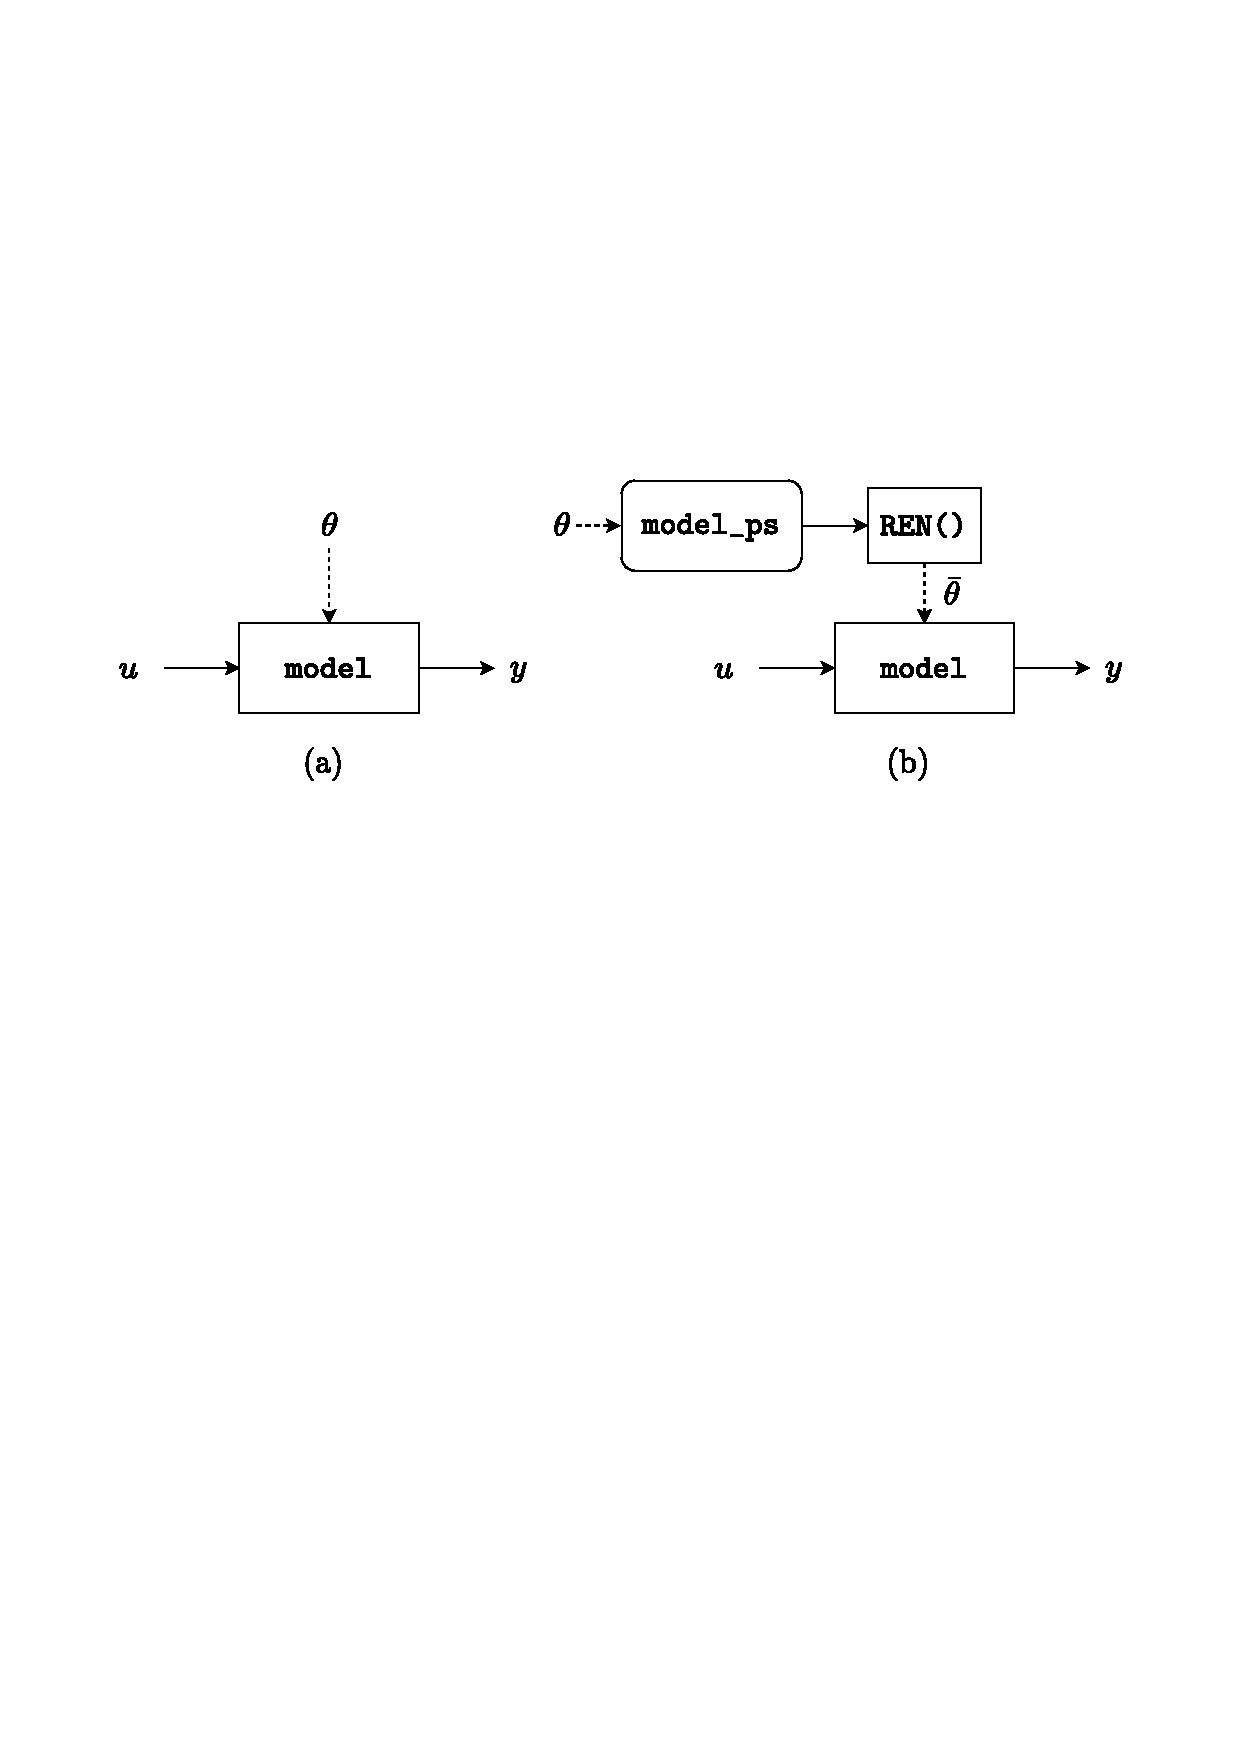
\includegraphics[width=0.45\textwidth]{Images/rrn_julia_params.pdf}
    \caption{Association of models and their parameters in (a) \texttt{Flux.jl} and (b) \texttt{RobustNeuralNetworks.jl}. In (a), model parameters $\theta$ are associated with the \texttt{model}. In (b), the direct parameters $\theta$ are associated with the parameterization \texttt{model\_ps}, and are converted to explicit parameters $\bar{\theta}$ when the \texttt{model} is constructed for evaluation with \texttt{REN()}.}
    \label{fig:ren-params}
\end{figure}

% Parameterisation types
\subsubsection{Types of direct parameterizations} \label{sec:direct-params}

There are currently four REN parameterizations implemented in this package:
\begin{enumerate}
    \item \verb|ContractingRENParams| parameterizes contracting RENs with a user-defined upper bound on the contraction rate.

    \item \verb|LipschitzRENParams| parameterizes RENs with a user-defined (or learnable) Lipschitz bound $\gamma \in (0,\infty)$.

    \item \verb|PassiveRENParams| parameterizes incrementally input passive RENs with user-tunable passivity parameter $\nu \ge 0$.

    \item \verb|GeneralRENParams| parameterizes RENs satisfying some general behavioural constraints defined by an incremental IQC with parameters (Q,S,R).
    
\end{enumerate}

There is currently one LBDN parameterization implemented in \verb|RobustNeuralNetworks.jl|:

\begin{enumerate}
    \item \verb|DenseLBDNParams| parameterizes dense (fully-connected) LBDNs with a user-defined or learnable Lipschitz bound. A dense LBDN is effectively a Lipschitz-bounded MLP.
\end{enumerate}

We intend to add \verb|ConvolutionalLBDNParams| to parameterize the convolutional LBDNs in \cite{Wang+Manchester2023} in future iterations of the package.

% Explicit model wrappers
\subsubsection{Explicit model wrappers} \label{sec:explicit-wrappers}

When training a REN or LBDN, we learn and update the direct parameters $\theta$ and convert them to the explicit parameters $\bar{\theta}$ only for model evaluation. The main constructors for explicit models are \verb|REN| and \verb|LBDN|.

Users familiar with \verb|Flux.jl| will be used to creating a model once and then training it on their data. The typical workflow is as follows.

\begin{lstlisting}[language = Julia]
using Flux

# Define a model and a loss function
model = Flux.Chain(
    Flux.Dense(1 => 10, Flux.relu), 
    Flux.Dense(10 => 1, Flux.relu)
)

loss(model, x, y) = Flux.mse(model(x), y)

# Training data of 20 batches
T = Float32
xs, ys = rand(T,1,20), rand(T,1,20)
data = [(xs, ys)]

# Train the model for 50 epochs
opt_state = Flux.setup(Adam(0.01), model)
for _ in 1:50
    Flux.train!(loss, model, data, opt_state)
end
\end{lstlisting}

When training a model constructed from \verb|REN| or \verb|LBDN|, we need to back-propagate through the mapping from direct (learnable) parameters to the explicit model. We must therefore include the model construction as part of the loss function. If we do not, then the auto-differentiation engine has no knowledge of how the model parameters affect the loss, and will return zero gradients. Here is an example with an \verb|LBDN|, where the \verb|model| is defined by the direct parameterization stored in \verb|model_ps|.

\begin{lstlisting}[language = Julia]
using Flux, RobustNeuralNetworks

# Define model parameterization and loss function
T = Float32
model_ps = DenseLBDNParams{T}(1, [10], 1; nl=relu)
function loss(model_ps, x, y) 
    model = LBDN(model_ps)
    Flux.mse(model(x), y)
end

# Training data of 20 batches
xs, ys = rand(T,1,20), rand(T,1,20)
data = [(xs, ys)]

# Train the model for 50 epochs
opt_state = Flux.setup(Adam(0.01), model_ps)
for _ in 1:50
    Flux.train!(loss, model_ps, data, opt_state)
end
\end{lstlisting}

% Why separate models
\subsubsection{Separating parameters and models} \label{sec:separate-params}

For the sake of convenience, we have included the model wrappers \verb|DiffREN| and \verb|DiffLBDN| as alternatives to \verb|REN| and \verb|LBDN|, respectively. These wrappers compute the explicit parameters each time the model is called rather than just once when they are constructed. Any model created with these wrappers can therefore be used exactly the same way as a regular \verb|Flux.jl| model, and there is no need for model construction in the loss function. One can simply replace the definition of the \verb|Flux.Chain| model in the \verb|Flux.jl| example with
\begin{lstlisting}[language = Julia]
model_ps = DenseLBDNParams{T}(1, [10], 1; nl=relu)
model = DiffLBDN(model_ps)
\end{lstlisting}
and train the LBDN just like any other \verb|Flux.jl| model. We use these wrappers in Sections \ref{sec:mnist} and \ref{sec:observer}.

The trade-off in using \verb|DiffREN| or \verb|DiffLBDN| is computational efficiency in applications where a model is called many times before a training update (e.g., reinforcement learning). The main computational bottleneck in training a REN or LBDN is converting from the direct to explicit parameters (mapping $\theta \mapsto \bar{\theta}$). This process involves a matrix inverse where the number of matrix elements scales quadratically with the dimension of the model in a REN or the dimension of each layer in an LBDN (see \cite{Revay++2023,Wang+Manchester2023}). If a model is to be evaluated many times with the same direct parameters in between training updates, it is more efficient to compute the explicit parameters once, hold them fixed over many model calls, and only re-compute them once the direct parameters have been updated. This is exactly the purpose of keeping \verb|model_ps| and \verb|model| separate when using \verb|REN| and \verb|LBDN|. Note that we cannot store the direct and explicit parameters in the same \verb|model| object since auto-differentiation in Julia does not support array mutation \cite{Innes2018b}. We therefore advise using \verb|DiffREN| or \verb|DiffLBDN| for convenience in applications where the model parameters are updated after just one model call (e.g., training an image classifier). The computational benefits of separating models from their parameterizations is explored numerically in Section \ref{sec:rl}.
